% Author: Till Tantau
% Source: The PGF/TikZ manual

\documentclass{article}

\usepackage{pgf}
\usepackage{tikz}
\usetikzlibrary{arrows,automata}
\usepackage[latin1]{inputenc}
\usepackage{verbatim}

\begin{document}

\begin{comment}
:Title: State machine
:Tags: Manual, Automata, Graphs

Another examle from the manual.

| Author: Till Tantau
| Source: The PGF/TikZ manual

\end{comment}

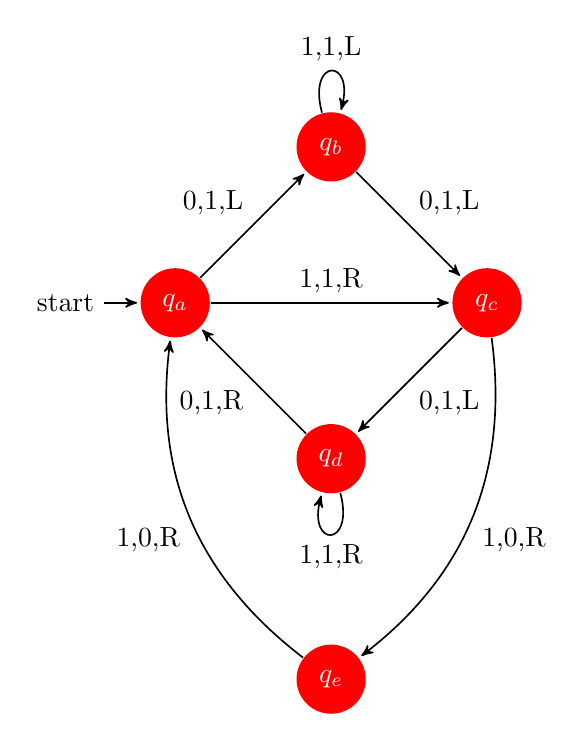
\begin{tikzpicture}[->,>=stealth',shorten >=1pt,auto,node distance=2.8cm,
                    semithick]
  \tikzstyle{every state}=[fill=red,draw=none,text=white]

  \node[initial,state] (A)                    {$q_a$};
  \node[state]         (B) [above right of=A] {$q_b$};
  \node[state]         (D) [below right of=A] {$q_d$};
  \node[state]         (C) [below right of=B] {$q_c$};
  \node[state]         (E) [below of=D]       {$q_e$};

  \path (A) edge              node {0,1,L} (B)
            edge              node {1,1,R} (C)
        (B) edge [loop above] node {1,1,L} (B)
            edge              node {0,1,L} (C)
        (C) edge              node {0,1,L} (D)
            edge [bend left]  node {1,0,R} (E)
        (D) edge [loop below] node {1,1,R} (D)
            edge              node {0,1,R} (A)
        (E) edge [bend left]  node {1,0,R} (A);
\end{tikzpicture}

\end{document}